\chapter{Setup for high resolution imaging}

\section{Experimental requirements}
\todo{cite marc repp for setup}
\subsection{Experimental setup}
	The atoms in our trap are confined in a vacuum chamber, which has windows in x,y and z direction for the incident lasers, to either trap or image the atoms in the centre. The double species camera (Andor iKon M) is placed along the z axis, above the chamber on a breadboard, where it is also possible to switch to another camera.
	
	A bikonvex lens focuses the imaging beam onto the CCD camera. To minimize the incident background light, the imaging path is covered in SM3 tubes, which can be directly connected to the camera due to a custom made front panel (see Appendix image). \todo{Appendix image}
	\todo{cite carmen}
	
	The camera is also very sensitive to stray light, so that it has to be protected between measurements with a shutter, that covers the front end of the imaging path, such that no light will enter the camera, which will be covered in more detail in \refSec{shutter}
	
	\draft{imaging_path}{Imaging path}{The camera stands on a breadboard, together with the mirrors, the lens and the SM3 tube. The imaging beam originates from the z-axis (pointing out of the document), then transversing as shown.}

\subsection{Basics of CCD cameras}
\label{ch:ccd_basics}
	
	Cameras operate by means of converting photons first into electrons then into voltage and finally read out as data. Each conversion process can add noise to the final image, which needs to be minimized in order to acquire accurate data, which will be covered in \refCh{camera}.
	
	The photons are collected on an array of semiconductors, called the pixels, where ideally the spacing between the pixels is zero to get maximum accuracy. The resolution is then dependent on the pixel size, which is for scientific cameras usually between \SI{10}{\micro\meter} and \SI{20}{\micro\meter} per pixel. Bigger pixels means higher photon sensitivity but usually lower resolution.
	
	To create the digital image, the pixels have to be shifted into the analog digital converter (ADC). This is done, by vertically shifting them into the readout register and then horizontal into the ADC, where the charges are multiplied and converted to digital data.
	
	\draft{ccd_shifts}{CCD scheme}{
		The pixels are arranged in the pixel array. During readout they are shifted upwards into the readout register and then to the side into the analog to digital converter
	}
	
	The shifting is done by storing the charges after collecting them. Each storage can be seen as an electronic potential. To successfully shift the charges and prevent overlapping, three potentials $U_1$, $U_2$ and $U_3$ are necessary. \refFig{charge_shift} indicates the systematics behind the shifting.
	
	\draft{charge_shift}{Shifting charges}{
		To shift charges from Pixel A to Pixel B, the potentials have to be set accordingly to allow the charge flow without overlapping each other. The drawing illustrates the charges moving from Pixel A to B, each row indicates the next step. Moving electrons to the next potential is a three-step process. The charges are first only present in the low potential $U_i$, while $U_{i+1}$ is kept high, then distributed across $U_i$ and $U_{i+1}$ by setting them both low and at last $U_i$ will be set high such that the charge is now fully in $U_{i+1}$.
	}
	
\subsection{Atom imaging} \todo{better title}
\todo{cite stephan helmrich}
\todo{cite simon murmann}
In order to find microscopic attributes of atoms, or systems of atoms, it is necessary to look at the atoms themselves. This is commonly accomplished using either fluorescence or absorption imaging. In both cases, a laser is pointed at an atomic cloud, that is cooled and confined in a trap. In fluorescence imaging, the experimentalist will look at the light, the cloud radiates, since it is illuminated by the incident light.
Naturally, the intensity from the light through this method is not very high, since it is radiated in all directions, but is nevertheless useful for single-atom detection.

In absorption imaging, the imaging system is parallel to the imaging beam. Without atoms, one would therefore see a beam profile of the laser, although with atoms, a shadow is visible due to the atoms blocking the light. This is accomplished, by correctly tuning the laser to a resonance frequency of the atoms, which enables them to absorb the light, exciting them to a higher state. Through spontaneous emission, the atoms will decay, making it possible to excite them once again. For a dense cloud, enough light is absorbed, such that the blocked light intensity differs enough to distinguish them from the laser profile.

\todo{example two level atom excitation image}

There are a set of optical elements in the imaging path, like lenses to collimate the image and refocus it, or mirrors to guide the light into the camera. Since the surfaces will most likely introduce errors into the imaging, for example from impurities or dust, only the absorption image will not suffice to gain reliable data. This is compensated by taking a total of three pictures, in order to extract only the relevant information from the image.

This can be understood when looking at the light intensity reaching the camera. The atom cloud has a optical density $OD$, therefore the intensity can be written as
\begin{equation}
I_{CCD} = I_0 e^{-OD} + I_{back},
\end{equation}
where the intensity decreases from the incident laser intensity $I_0$ as the optical density rises. The intensity $I_{back}$ contains statistical errors, that are found when the CCD is not being illuminated such as readout noise or dark noise. All the interesting attributes of atoms are found by looking at the optical density, therefore in order to extract that, a background frame is subtracted from the absorption image and the laser profile divided, leaving
\begin{equation}
\frac{I_{CCD} - I_{back}}{I_0} = e^{-OD}.
\end{equation}
The laser intensity $I_0$ has to be taken as a whole separate image, containing the laser intensiy $I_0'$ and also the background $I_{back}$, therefore the equation yields
\begin{equation}
\frac{I_{CCD} - I_{back}}{I_0' - I_{back}} = e^{-OD}.
\end{equation}
\todo{three images as example}
%cool reference: http://muellergroup.lassp.cornell.edu/basictraining2009/OpticalAbs.pdf
\todo{read comment}

From the resulting optical density, one can now conclude for example atom density distributions, atom numbers or excitation rates.
In the course of this thesis, the goal will be pursued to minimize all errors that can occur during acquisition. It will be seen, that features from the camera such as water cooling and quantum efficiency play a high role to accomplish that goal. Consequently, the next chapter is dedicated to the camera that will be used for future measurements.

\section{Camera for double species imaging}
\label{ch:camera}

\subsection{Comparison with the present setup}
For the application of imaging small atom clouds, it is very important to have cameras with optimal noise reduction and maximal readout speed. The new setup improves on both attributes, with the ability to cool the chip down to reduce the dark noise as well as the fast kinetics mode, making it possible to acquire all images before reading out, improving the speed at which images can be taken significantly.

The old setup used a Guppy-38B camera, which is a lot smaller than the Andor iKon M \todo{add reference to Marc Repp} (\SI{48.2x30x30}{\milli\meter} vs \SI{204.2x105x107}{\milli\meter}), therefore making an implementation on a full experimental table easier. To implement such a complicated camera system that the Andor is, a lot of prseparation was made in the thesis of Carmen. \todo{reference carmen}

Nevertheless, despite its size, the new camera offers the ability to image both Lithium and Caesium species at once, while two Guppy cameras were needed beforehand, which also meant placing them on different imaging axes.

When comparing the resolution, the chip size also has to be considered. Since higher resolutions seem to be preferable at first, it also means that for the same pixel sizes, the photon sensitivities will decrease. The pixel sizes compare to \SI{11}{\micro\meter} to \SI{13}{\micro\meter} from the old versus the new setup respectively, while the resolutions are \SI{768x492}{} and \SI{1024x1024}{} making a larger magnification now possible.
\todo{would be great to have maybe an image of the atoms with the old and new setup (maybe same cooling steps etc.)}

As already mentioned, the readout speed is highly important in our setup. Since absorption imaging is the technique of choice to measure atom attributes, three images need to be taken each sequence, being the absorption, division and background image.
For the Guppy camera, at a frame rate of 30fps, this meant the acquisition was finished after \SI{100}{\milli\second}. The Andor camera, on the other hand, can take images quickly without the need to read out in-between. At the fastest shift speed, the acquisition is finished after \SI{1.2}{\milli\second}, improving the speed by a factor of almost $100$.

\subsection{Dark current}
\todo{cite, see comment}
%http://www.kip.uni-heidelberg.de/matterwaveoptics/publications/theses/diplom_ottenstein.pdf
%http://www.mpia.de/AO/INSTRUMENTS/FPRAKT/4_F36_CCDscript2011.pdf
A common noise source that is apparent in all CCD cameras, is the so-called dark current. This noise accumulates seemingly random on the pixels, distributing the electron counts gaussian.

It originates from the nature of the pixels. Since they are made of semiconductors, once in a while, an electron can pass the potential between valence and conduction band simply due to thermal energy.

Luckily, the noise has a strong temperature dependece found from
\begin{equation}
I_{dark}(T) \propto T^{\frac{3}{2}} \mathrm{exp}(-E_g/2k_BT),
\end{equation}
while $E_g$ is the potential in the semiconductor, $T$ the temperature and the Boltzmann constant $k_B$.
Therefore in order to reduce dark current noise, the temperature of the chip can be reduced, therefore decreasing the thermal energy of the electrons.

This has been measured and verified in \refFig{electrpp}, using the built-in peltier element in the Andor camera.

When acquiring images with a high temperature, the dark current accumulating on the chip can be seen uniformly, adding a common offset to the pixels. Together with the finite readout speed, a gradient is visible on the chip, as dark current is still apparent on pixels that have not yet been read out. Therefore the first pixel will have fewer counts as the last pixel.
This can be seen for example in \todo{add a figure for the gradient}.

\plt[true]{electrpp}{Dark noise}{
	The dark noise follows a power law dependency. Since these measurements were taken without water cooling installed, deviations are visible as the temperature reaches \SI{-70}{\degreeCelsius}. The convergence to zero on the counts and their variance indicates accurate imaging when low temperatures are used. Gain in this measurement was minimal and the exposure time set to \SI{100}{\second}, such that dark current was the dominant noise source.
}

\newpage
\subsection{Readout noise}
%http://www.mssl.ucl.ac.uk/www_detector/ccdgroup/optheory/ccdoperation.html
As seen in \refCh{ccd_basics}, pixels get shifted in order to be read out. Moving charges from pixel to pixel causes noise to accumulate over each iteration. In theory, this is visible as a gradient since each shift adds new charges due to excitations in the semiconductors. A possible characterization of this effect is to simply take the variance of an image.

Although the shifting gradient is not visible in the final picture, since it is removed by subtracting the background image, it is still important to minimize the noise originating from shifting the charges, which was found to be the case for slow readout speeds, see \refFig{hvspeed}.

\plt{hvspeed}{Readout noise}{
	The pixels are shifted row-wise into the readout register, depending on the vertical shift speed ($v_{ss}$) and then moved pixel-by-pixel with the horizontal shift speed into the analog to digital converter. Since noise reduction is important, minimal horizontal shift speeds will be used, while the vertical shift speed does not seem to affect the variance. To make the readout the dominant noise source, temperature was set to \SI{-69}{\degreeCelsius} and exposure to \SI{10}{\milli\second}.
}
\todo{Add reference}

This is intuitive, since shifting charges means increasing and decreasing potential wells, so that they can move from one into the other. If this is done fast enough, electrons are more likely to excite others from the valence to the conduction band, therefore adding noise.

\newpage
\subsection{Quantum efficiency}
When selecting cameras for scientific imaging, one of the attributes to look out for is quantum efficiency. Not all incoming photons are converted into electrons, which adds an uncertainty into measurements. Therefore quantum efficiency is introduced, to describe the uncertainty mathematically, so that it is defined as the fraction of photons that are converted into electrons. A quantum efficiency $QE$ of 100\% would therefore mean, that every incident photon is detected on the chip. This can be put into equations as
\begin{equation}
QE = \frac{N_{detected}}{N_{total}}.
\end{equation}

The measurement of the quantum efficiency has been previously carried out by Carmen Renner \todo{cite} in her diploma thesis. In order to do that, the detected photons can be rewritten according to \todo{murmann}:
\begin{equation}
N_{total} = \frac{E_{beam}}{E_\gamma} = \frac{P t_{exp}}{E_\gamma}
\end{equation}
using the energy of all photons reaching the camera $E_{beam}$ which is described as using the power $P$ and exposure time $t_{exp}$. The photon energy $E_\gamma$ is calculated from $E_\gamma= h\nu$.

Now the quantum efficiency reads as
\begin{equation}
QE = \frac{h \nu N_{detected}}{P t_{exp}}.
\end{equation}
A measurement can therefore be carried out by plotting the accumulated counts against the exposure time, yielding the quantum efficiency, which was measured as \todo{make this sentence right} for \SI{852}{\nano\meter} and for \SI{671}{\nano\meter} light.

This camera was especially chosen from the quantum efficiency, since it is important in our case, to be able to detect most photons from Lithium and Caesium absorption.

\subsection{Pixel correlations}
\begin{itemize}
	\item Mainly the measurement (TBD)
	\item Some example images here maybe?
\end{itemize}

\section{Mechanical shutter}
\label{sec:shutter}

\subsection{Electronic setup}
\label{subsec:shutter_electronic}
\todo{headline}
\todo{cite andor manual somewhere}

The Andor camera has a very sensitive chip, which needs to be protected. In order to not unnecessarily illuminate the chip between measurements, a shutter is built into the optical path, which can also be seen in \refFig{imaging_path}. The shutter has five fans, as seen in \todo{appendix image}, which are mechanically guided, such that they together perform a circular motion outwards. The circular motion is best achieved for narrow fans, therefore needing more in order to close the shutter properly.

The guides are connected to each other and can be pulled outwards with a mechanical switch, that can be manually pushed or pulled. To drive the shutter electronically, a magnetic coil and a magnet are used. When the coil receives a current, the magnet, which is connected to the switch will pull the guides, moving them outwards, therefore opening the shutter.

Although the coil can pull the magnet in, it cannot be pushed away. This is compensated using a spring, which is connected to the switch. This also means, that the current driving the coil needs to be high enough, to also work against the spring.

The most optimal case would be now to have fast opening and closing times, since again we want to prevent illumation between measurements. This can be achieved by testing several springs and to make the pull from the magnetic coils as fast as possible, which means increasing the current to drive it. To achieve the latter, a custom circuit is used, as outlined in \refFig{shutter_circuit_simplified}.

The springs were tested in \refSubsec{shutter_dynamical}, and were found to be a substantial part in the setup.

\pltCustom{
	\begin{center}
		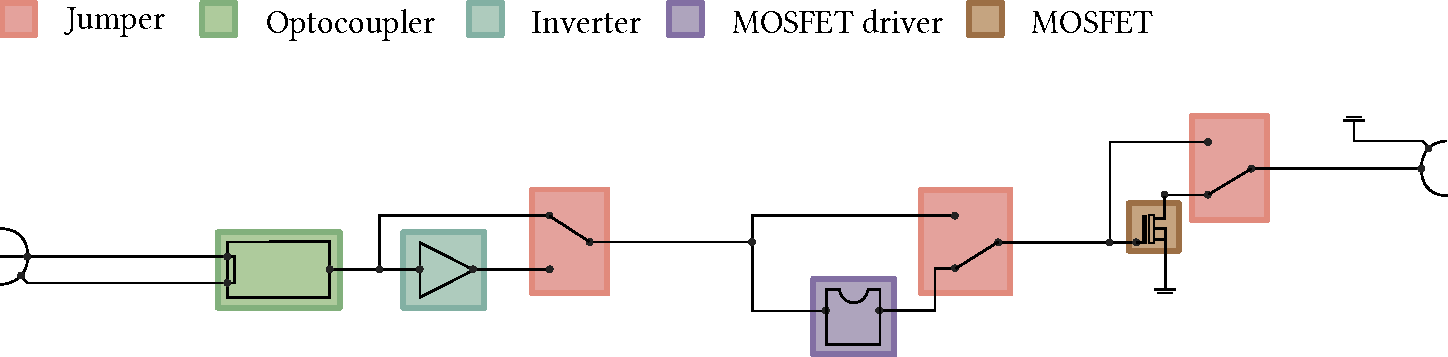
\includegraphics[width=1\textwidth]{drafts/shutter_circuit_simplified.pdf}
	\end{center}
}{shutter_circuit_simplified}{Simplified circuit to control the shutter}{
The mechanical shutter has to have a high amplitude input, in order to open as fast as possible. To achieve that, a metal–oxide–semiconductor field-effect transistor (or short, MOSFET) is used.
The experiment uses several magnetic fields, so that it is mandatory to decouple parts from the circuit, in order to not create loops, which would induce charges. This is achieved using the optocoupler.
Apart from that, all remaining parts in this curcuit are optional, as they can be skipped, by setting the jumpers that are highlighted in red. The inverter will flip the sign on the voltage. The MOSFET driver is used in order to serve the correct voltage at the transistor's gate and to help during discharge, such that the MOSFET will not overheat. The transistor will finally serve a high current \SI{2}{\ampere}, that is ouptput to the shutter.
The jumpers in this figure are set as they are used in the experiment.
}
\todo{appendix}
\todo{verify current}

\newpage
\subsection{Dynamical properties}
It was discussed before, in \refSubsec{shutter_electronic}, that more fans give a better approximation to a circular motion. Optimally, we would expect the shutter to open perfectly circular with linear velocity.

In order to find the actual dynamics of the shutter, an experiment was set up. The shutter was probed at several positions, using a laser, to find the opening time. An example of one of many measurements is shown in \refFig{shutterOpen}.

The points have been found using a photo diode on the other side of the shutter. Since the laser has a finite radius, there is a transition in the signal from the minimum to the maximum, which is due to the approximately linear opening velocity of the shutter and the gaussian intensity distribution of the laser beam.


\plt{shutterDiodeSignal}{
	Shutter characterization}{The dynamics of the shutter were measured using a laser with a variable horizontal offset, which is fixed in this plot, and a photo diode measuring the laser intensity. For various offsets, error functions were fitted yielding the time until the shutter opens to this offset. The opening time was hereby defined, where the error function has its mean value.
}

\todo{appendix image}
\plt{shutterOpen}{Sample dynamics}{
	Opening velocity was measured using the beam diameter and the time the shutter needed to transverse it. For each offset, a set of ~100 images were taken and the errors found as being the variance. It is noticeable, that the opening velocity on the right side is faster at first than on the left side. This is due to the structure of the shutter, as can be seen in [Appendix image of shutter].
	The overall opening speed on the other hand is not affected by this and seems to be linear with the offset.
}

The characterization of the shutter is indeed very important, since then the acquisitions can be accurately timed when the shutter is fully open. But in order to optimize it, there were two shutters at hand, and several springs to choose from. Each combination was tested carefully and it was found, that opening and closing of the shutter are connected. This is a consequence of the mechanics, where the several springs have a higher force, therefore closing faster, but making it more difficult for the coil to pull the magnet in, to open it. 
\newpage
\section{Mask for the CCD sensor}
\subsection{Fast kinetics mode}
\label{ch:fast_kin}
%\begin{itemize}
%	\item Why it is good
%	\item Shifting timescales
%\end{itemize}
The experiment needs to image both Lithium and Caesium back to back as fast as possible, so that the system does not change significantly during the acquisition of both species.

As explained earlier in \refCh{ccd_basics}, the readout consists of first shifting a row into the readout register and then horizontally shifting them into the ADC. This is a very time consuming process, since the total readout time is described by
\begin{equation}
t_{ij} = i*vspeed + (i-1)*j_{max}*hspeed+j*hspeed
\end{equation}
This equation describes a readout process until a pixel with the coordinates $i$ and $j$, where readout of all pixels beforehand is also taken into account, hence the $j_{max}$ which is the width of the chip in pixels.
As can be seen, for the terms of the horizontal speed, the pixel position has for the last pixel in a row a quadratic dependency, being the dominant terms for the readout, which is necessary to shift the pixels into the ADC.

Therefore, the fast kinetics mode allows the image acquisition to be only dependant on the vertical shift speed, reducing the acquisition time significantly. Only a portion of the CCD is illuminated, while the dark parts of the chip will be used as a storage. This means, that as soon as an image is taken, the illuminated pixels are shifted vertically behind a mask, such that no photons can reach them any more. When the chip is then full or the user has finished their acquisition, the known readout process is then started, including the shift into the ADC, at which point the speed should not matter too much any more, because the experiment is then finished.

\pltCustom{
	\begin{center}
		\begin{overpic}[width=0.5\textwidth]{drafts/fast_kinetics.pdf}
			\put (-6,92) {\textbf{a.}}
			\put (41,92) {\textbf{b.}}
			\put (58,92) {\textbf{c.}}
			\put (5,44) {\textbf{d.}}
			\put (27,44) {\textbf{e.}}
			\put (49,44) {\textbf{f.}}
			\put (69,44) {\textbf{g.}}
		\end{overpic}
	\end{center}
}{fast_kinetics}{Schematics of fast kinetics mode}{
\textbf{a.}\enskip Laser photons excite electrons in the pixel, creating the first absorption image.
\textbf{b.}\enskip The illuminated pixels are shifted down behind the cover of the slit, while the laser is shut off.
\textbf{c.}\enskip The second absorption image is taken without affecting the last measurement.
\textbf{d.}\enskip Both images are shifted down before starting the readout process, to not falsify the data with stray light.
\textbf{e.}\enskip The readout process starts, the first row is shifted into the readout register.
\textbf{f.}\enskip The first pixels are shifted into the ADC.
\textbf{g.}\enskip Step e. to f. are repeated until the chip is cleared.
}

To set up the fast kinetics mode, there are several parameters that need to be set in advance.
\begin{itemize}
	\item \textbf{Series length}\, The number of images acquired before the readout phase is initiated.
	\item \textbf{Exposed rows}\, The height of an image in the fast kinetic series.
	\item \textbf{Offset from bottom}\, Number of rows below each image which is not read out due to diffraction effects of the masking setup which have to be discarded anyway, see \refSubsec{slit}.
\end{itemize}

It can be already seen, that the parameters are limited by the height of the CCD in pixels:
%The CCD has a pixel height of \SI{1024}{\px}, such that the condition
\begin{equation}
\mathbf{Series\,length} * (\mathbf{Exposed\,rows} + \mathbf{Offset\,from\,bottom}) \leq \SI{1024}{px}
\end{equation}
We find it optimal for our application, to expose \SI{200}{\px}, therefore giving a series length of $5$ and an offset of \todo{offset?}. This is since we will be imaging two species, therefore taking an absorption image for each species, followed by two division images, one for each species. The fifth image is left empty, since it would be illuminated during readout, therefore falsifying the data as stated in \refFig{fast_kinetics}. As a matter of fact, the fifth image is cropped out, so that it even the readout time.

\subsection{Frequency response of a slit}
\label{subsec:slit}

In the previous section, the fast kinetics mode was introduced as well as the experimental setup required. The slit in front of the camera is yet another optical element in the path, which will introduce diffraction on the chip - an effect due to the wave nature of light.
\refFig{slit_sketch} is a sketch of the systematics behind a laser wave approaching a slit.

\draft{slit_sketch}{Diffraction on a single slit}{A planar wave with the wavelength $\lambda$ approaches the slit having a width $a$, where the maxima of the wave are drawn as dashed lines. After the slit, Huygens principle is sketched as spherical waves, in purple and green, interfering with each other, which is described in more detail below. The new wavefront is therefore where the 	waves cross each other and is as such visible on the screen to the right.}

The incoming planar wave can be described by the formula:
\begin{equation}
E(x,z) = E_0 e^{-ikz},
\end{equation}
where the wave is propagating in the $z$-Direction with the wave number $k$ and an amplitude $E_0$.

It is known from Huygens principle, that each point from a planar wave can be seen as the origin of a spherical wave. The spherical waves will interfere with each other, making use of the superposition principle and therefore building up the new wavefront.

\todo{reference d. steck}
The mathematical formalism of Huygens principle is simply the sum of all spherical waves, which is for infinitely small distances given as:
\begin{equation}
E(x,z) = E_0 C \int_{Slit} \frac{1}{r^2} \mathrm{exp}(-ikr)\mathrm{d}x'.
\end{equation}
Here, $r=\sqrt{(x-x')^2 + z^2}$ is the radius of a two dimensional wave, C is a normalization constant.
Taylor expansion allows us, to substitute $r^2$ with $z^2$ and $r$ with $\frac{(x-x')^2}{2z} + z^2$, while also the approximation $(x-x') \ll z$ needs to be fulfilled. Therefore we get:
\begin{equation}
E(x,z) = E_0 e^{-ikz}\sqrt{\frac{ik}{2\pi z}}\int_{Slit} \mathrm{exp}(-\frac{ik}{2z}(x-x')^2)\mathrm{d}x'.
\end{equation}
The normalization was derived from the gaussian normal distribution. The integral will run over the slit size, with the origin in its middle, the width being $a$.
We want to also write the exponential as a function of $-\frac{i\pi t^2}{2}$, due to the definition of fresnel integrals. The substitution follows:
\begin{equation}
\frac{k}{2z}(x-x')^2 = \frac{\pi t^2}{2},
\end{equation}
\begin{equation}
\Rightarrow t = \sqrt{\frac{k}{z\pi}}(x-x'), \\
\end{equation}
\begin{equation}
\Rightarrow \mathrm{d}x' = -\mathrm{d}t \sqrt{\frac{z\pi}{k}},
\end{equation}
such that the field becomes
\begin{equation}
E(x,z) = -E_0 e^{-ikz}\sqrt{\frac{i}{2}}\int_{t(-a/2)}^{t(a/2)} \mathrm{exp}(-\frac{i\pi t^2}{2})\mathrm{d}t.
\end{equation}
The fresnel integrals are defined by
\begin{equation}
C(x) = \int_0^x \mathrm{cos}(\frac{\pi t^2}{2})\mathrm{d}t,
\end{equation}
\begin{equation}
S(x) = \int_0^x \mathrm{sin}(\frac{\pi t^2}{2})\mathrm{d}t,
\end{equation}

so that in combination with Eulers equations and splitting up the integrals the equation for the electric field is:
\begin{equation}
E(x,z) = E_0 \sqrt{\frac{i}{2}} e^{-ikz} \left [ C(-a/2) - C(a/2) - iS(-a/2) + iS(a/2) \right ].
\end{equation}

In a real experiment, the light would fall on a CCD chip with its electric field $E(x,z)$, while the representation would later be the intensity, which is given by
\begin{equation}
I(x,z) = \frac{2 \lvert E(x,z) \rvert ^2}{\epsilon_0 c} ,
\end{equation}
with the dielectric constant $\epsilon_0$ and the speed of light $c$.

To verify the theory, we set up a simple experiment with a collimated laser beam pointing at the CCD of the Andor camera, with a slit in between, the results of which can be seen in \refFig{slit}.

\plt{slit}{Diffraction measurement}{
	In order to characterize the diffraction on the CCD, a slit was placed as close as possible. The parameters were then measured as distance $d=\SI{10.9}{\milli\meter}$, opening $a=\SI{2.5}{\milli\meter}$ using a ruler, therefore limiting the accuracy to \SI{0.5}{\milli\meter}. The wavelength was $\lambda =\SI{852}{\nano\meter}$ found from the laser specifications. The blue curve is the experimental data, while the red curve was fitted, leaving distance and opening free. They were found to be $d^\prime=\SI{11.0\pm0.3}{\milli\meter}$ and $a^\prime=\SI{2.470\pm0.013}{\milli\meter}$, which is in close agreement. The laser does not have a constant intensity over the chip size, therefore deviations in amplitude are visible.
}

Apparently, the theory matches the experiment very well, since the deviations are in the expected regimes.
The function washes out as it approaches the centre of the chip. This is due to the nature of the pixels, which only have a finite size and the fact, that the frequencies of the oscillations are lower on the outer ends. All oscillations that fit into one pixel are averaged, therefore diffraction is not visible and it can be said that the data is accurate.

A further experiment has been deduced to also find a relation of the frequencies to the slit distance, which can be seen in \refFig{slit_scheme}.

\pltCustom{
	\begin{overpic}[width=0.5\textwidth]{drafts/slit_scheme.pdf}
		\put (1,67) {\textbf{a.}}
	\end{overpic}
	%% Creator: Matplotlib, PGF backend
%%
%% To include the figure in your LaTeX document, write
%%   \input{<filename>.pgf}
%%
%% Make sure the required packages are loaded in your preamble
%%   \usepackage{pgf}
%%
%% Figures using additional raster images can only be included by \input if
%% they are in the same directory as the main LaTeX file. For loading figures
%% from other directories you can use the `import` package
%%   \usepackage{import}
%% and then include the figures with
%%   \import{<path to file>}{<filename>.pgf}
%%
%% Matplotlib used the following preamble
%%   \usepackage{fontspec}
%%   \setmainfont{DejaVu Serif}
%%   \setmonofont{DejaVu Sans Mono}
%%
\begingroup%
\makeatletter%
\begin{pgfpicture}%
\pgfpathrectangle{\pgfpointorigin}{\pgfqpoint{3.390000in}{2.095135in}}%
\pgfusepath{use as bounding box, clip}%
\begin{pgfscope}%
\pgfsetbuttcap%
\pgfsetmiterjoin%
\definecolor{currentfill}{rgb}{1.000000,1.000000,1.000000}%
\pgfsetfillcolor{currentfill}%
\pgfsetlinewidth{0.000000pt}%
\definecolor{currentstroke}{rgb}{1.000000,1.000000,1.000000}%
\pgfsetstrokecolor{currentstroke}%
\pgfsetdash{}{0pt}%
\pgfpathmoveto{\pgfqpoint{0.000000in}{0.000000in}}%
\pgfpathlineto{\pgfqpoint{3.390000in}{0.000000in}}%
\pgfpathlineto{\pgfqpoint{3.390000in}{2.095135in}}%
\pgfpathlineto{\pgfqpoint{0.000000in}{2.095135in}}%
\pgfpathclose%
\pgfusepath{fill}%
\end{pgfscope}%
\begin{pgfscope}%
\pgfsetbuttcap%
\pgfsetmiterjoin%
\definecolor{currentfill}{rgb}{1.000000,1.000000,1.000000}%
\pgfsetfillcolor{currentfill}%
\pgfsetlinewidth{0.000000pt}%
\definecolor{currentstroke}{rgb}{0.000000,0.000000,0.000000}%
\pgfsetstrokecolor{currentstroke}%
\pgfsetstrokeopacity{0.000000}%
\pgfsetdash{}{0pt}%
\pgfpathmoveto{\pgfqpoint{0.594467in}{0.451335in}}%
\pgfpathlineto{\pgfqpoint{3.191321in}{0.451335in}}%
\pgfpathlineto{\pgfqpoint{3.191321in}{1.923551in}}%
\pgfpathlineto{\pgfqpoint{0.594467in}{1.923551in}}%
\pgfpathclose%
\pgfusepath{fill}%
\end{pgfscope}%
\begin{pgfscope}%
\pgfpathrectangle{\pgfqpoint{0.594467in}{0.451335in}}{\pgfqpoint{2.596854in}{1.472216in}} %
\pgfusepath{clip}%
\pgfsetrectcap%
\pgfsetroundjoin%
\pgfsetlinewidth{0.501875pt}%
\definecolor{currentstroke}{rgb}{0.000000,0.750000,0.750000}%
\pgfsetstrokecolor{currentstroke}%
\pgfsetdash{}{0pt}%
\pgfpathmoveto{\pgfqpoint{0.592469in}{0.503172in}}%
\pgfpathlineto{\pgfqpoint{0.618438in}{0.516368in}}%
\pgfpathlineto{\pgfqpoint{0.644406in}{0.531872in}}%
\pgfpathlineto{\pgfqpoint{0.670375in}{0.549626in}}%
\pgfpathlineto{\pgfqpoint{0.696343in}{0.570729in}}%
\pgfpathlineto{\pgfqpoint{0.722312in}{0.595841in}}%
\pgfpathlineto{\pgfqpoint{0.748280in}{0.625553in}}%
\pgfpathlineto{\pgfqpoint{0.774249in}{0.660289in}}%
\pgfpathlineto{\pgfqpoint{0.800218in}{0.699456in}}%
\pgfpathlineto{\pgfqpoint{0.826186in}{0.745404in}}%
\pgfpathlineto{\pgfqpoint{0.852155in}{0.799263in}}%
\pgfpathlineto{\pgfqpoint{0.878123in}{0.862543in}}%
\pgfpathlineto{\pgfqpoint{0.904092in}{0.933088in}}%
\pgfpathlineto{\pgfqpoint{0.930060in}{1.011349in}}%
\pgfpathlineto{\pgfqpoint{0.956029in}{1.098093in}}%
\pgfpathlineto{\pgfqpoint{0.981997in}{1.194130in}}%
\pgfpathlineto{\pgfqpoint{1.007966in}{1.299556in}}%
\pgfpathlineto{\pgfqpoint{1.033934in}{1.406587in}}%
\pgfpathlineto{\pgfqpoint{1.059903in}{1.515480in}}%
\pgfpathlineto{\pgfqpoint{1.085872in}{1.619221in}}%
\pgfpathlineto{\pgfqpoint{1.111840in}{1.714344in}}%
\pgfpathlineto{\pgfqpoint{1.137809in}{1.794791in}}%
\pgfpathlineto{\pgfqpoint{1.163777in}{1.846792in}}%
\pgfpathlineto{\pgfqpoint{1.189746in}{1.879956in}}%
\pgfpathlineto{\pgfqpoint{1.215714in}{1.891007in}}%
\pgfpathlineto{\pgfqpoint{1.241683in}{1.870535in}}%
\pgfpathlineto{\pgfqpoint{1.267651in}{1.819844in}}%
\pgfpathlineto{\pgfqpoint{1.293620in}{1.744212in}}%
\pgfpathlineto{\pgfqpoint{1.319588in}{1.641192in}}%
\pgfpathlineto{\pgfqpoint{1.345557in}{1.524798in}}%
\pgfpathlineto{\pgfqpoint{1.371526in}{1.417361in}}%
\pgfpathlineto{\pgfqpoint{1.397494in}{1.333977in}}%
\pgfpathlineto{\pgfqpoint{1.423463in}{1.293682in}}%
\pgfpathlineto{\pgfqpoint{1.449431in}{1.303734in}}%
\pgfpathlineto{\pgfqpoint{1.475400in}{1.358742in}}%
\pgfpathlineto{\pgfqpoint{1.501368in}{1.450054in}}%
\pgfpathlineto{\pgfqpoint{1.527337in}{1.550051in}}%
\pgfpathlineto{\pgfqpoint{1.553305in}{1.641919in}}%
\pgfpathlineto{\pgfqpoint{1.579274in}{1.701164in}}%
\pgfpathlineto{\pgfqpoint{1.605242in}{1.704601in}}%
\pgfpathlineto{\pgfqpoint{1.631211in}{1.657776in}}%
\pgfpathlineto{\pgfqpoint{1.657179in}{1.572671in}}%
\pgfpathlineto{\pgfqpoint{1.683148in}{1.477269in}}%
\pgfpathlineto{\pgfqpoint{1.709117in}{1.406004in}}%
\pgfpathlineto{\pgfqpoint{1.735085in}{1.391625in}}%
\pgfpathlineto{\pgfqpoint{1.761054in}{1.437446in}}%
\pgfpathlineto{\pgfqpoint{1.787022in}{1.522033in}}%
\pgfpathlineto{\pgfqpoint{1.812991in}{1.609201in}}%
\pgfpathlineto{\pgfqpoint{1.838959in}{1.661373in}}%
\pgfpathlineto{\pgfqpoint{1.864928in}{1.649290in}}%
\pgfpathlineto{\pgfqpoint{1.890896in}{1.583976in}}%
\pgfpathlineto{\pgfqpoint{1.916865in}{1.502915in}}%
\pgfpathlineto{\pgfqpoint{1.942833in}{1.448209in}}%
\pgfpathlineto{\pgfqpoint{1.968802in}{1.458101in}}%
\pgfpathlineto{\pgfqpoint{1.994771in}{1.524472in}}%
\pgfpathlineto{\pgfqpoint{2.020739in}{1.604456in}}%
\pgfpathlineto{\pgfqpoint{2.046708in}{1.645356in}}%
\pgfpathlineto{\pgfqpoint{2.072676in}{1.621496in}}%
\pgfpathlineto{\pgfqpoint{2.098645in}{1.552345in}}%
\pgfpathlineto{\pgfqpoint{2.124613in}{1.491152in}}%
\pgfpathlineto{\pgfqpoint{2.150582in}{1.493047in}}%
\pgfpathlineto{\pgfqpoint{2.176550in}{1.548587in}}%
\pgfpathlineto{\pgfqpoint{2.202519in}{1.619896in}}%
\pgfpathlineto{\pgfqpoint{2.228487in}{1.648320in}}%
\pgfpathlineto{\pgfqpoint{2.254456in}{1.605986in}}%
\pgfpathlineto{\pgfqpoint{2.280424in}{1.544261in}}%
\pgfpathlineto{\pgfqpoint{2.306393in}{1.518762in}}%
\pgfpathlineto{\pgfqpoint{2.332362in}{1.555353in}}%
\pgfpathlineto{\pgfqpoint{2.358330in}{1.622765in}}%
\pgfpathlineto{\pgfqpoint{2.384299in}{1.646082in}}%
\pgfpathlineto{\pgfqpoint{2.410267in}{1.609514in}}%
\pgfpathlineto{\pgfqpoint{2.436236in}{1.560464in}}%
\pgfpathlineto{\pgfqpoint{2.462204in}{1.555772in}}%
\pgfpathlineto{\pgfqpoint{2.488173in}{1.608741in}}%
\pgfpathlineto{\pgfqpoint{2.514141in}{1.650250in}}%
\pgfpathlineto{\pgfqpoint{2.540110in}{1.638975in}}%
\pgfpathlineto{\pgfqpoint{2.566078in}{1.589263in}}%
\pgfpathlineto{\pgfqpoint{2.592047in}{1.568411in}}%
\pgfpathlineto{\pgfqpoint{2.618016in}{1.609322in}}%
\pgfpathlineto{\pgfqpoint{2.643984in}{1.650811in}}%
\pgfpathlineto{\pgfqpoint{2.669953in}{1.646970in}}%
\pgfpathlineto{\pgfqpoint{2.695921in}{1.605756in}}%
\pgfpathlineto{\pgfqpoint{2.721890in}{1.600687in}}%
\pgfpathlineto{\pgfqpoint{2.747858in}{1.644995in}}%
\pgfpathlineto{\pgfqpoint{2.773827in}{1.668609in}}%
\pgfpathlineto{\pgfqpoint{2.799795in}{1.649690in}}%
\pgfpathlineto{\pgfqpoint{2.825764in}{1.615546in}}%
\pgfpathlineto{\pgfqpoint{2.851732in}{1.636374in}}%
\pgfpathlineto{\pgfqpoint{2.877701in}{1.668414in}}%
\pgfpathlineto{\pgfqpoint{2.903670in}{1.667262in}}%
\pgfpathlineto{\pgfqpoint{2.929638in}{1.634292in}}%
\pgfpathlineto{\pgfqpoint{2.955607in}{1.636156in}}%
\pgfpathlineto{\pgfqpoint{2.981575in}{1.672242in}}%
\pgfpathlineto{\pgfqpoint{3.007544in}{1.676064in}}%
\pgfpathlineto{\pgfqpoint{3.033512in}{1.654885in}}%
\pgfpathlineto{\pgfqpoint{3.059481in}{1.650303in}}%
\pgfpathlineto{\pgfqpoint{3.085449in}{1.683497in}}%
\pgfpathlineto{\pgfqpoint{3.111418in}{1.682694in}}%
\pgfpathlineto{\pgfqpoint{3.137386in}{1.663554in}}%
\pgfpathlineto{\pgfqpoint{3.163355in}{1.665888in}}%
\pgfpathlineto{\pgfqpoint{3.189323in}{1.697600in}}%
\pgfpathlineto{\pgfqpoint{3.205210in}{1.692918in}}%
\pgfusepath{stroke}%
\end{pgfscope}%
\begin{pgfscope}%
\pgfpathrectangle{\pgfqpoint{0.594467in}{0.451335in}}{\pgfqpoint{2.596854in}{1.472216in}} %
\pgfusepath{clip}%
\pgfsetrectcap%
\pgfsetroundjoin%
\pgfsetlinewidth{0.501875pt}%
\definecolor{currentstroke}{rgb}{0.000000,0.000000,1.000000}%
\pgfsetstrokecolor{currentstroke}%
\pgfsetdash{}{0pt}%
\pgfpathmoveto{\pgfqpoint{0.592469in}{0.502138in}}%
\pgfpathlineto{\pgfqpoint{0.618438in}{0.516713in}}%
\pgfpathlineto{\pgfqpoint{0.644406in}{0.533762in}}%
\pgfpathlineto{\pgfqpoint{0.670375in}{0.553943in}}%
\pgfpathlineto{\pgfqpoint{0.696343in}{0.578800in}}%
\pgfpathlineto{\pgfqpoint{0.722312in}{0.608111in}}%
\pgfpathlineto{\pgfqpoint{0.748280in}{0.643120in}}%
\pgfpathlineto{\pgfqpoint{0.774249in}{0.684264in}}%
\pgfpathlineto{\pgfqpoint{0.800218in}{0.732476in}}%
\pgfpathlineto{\pgfqpoint{0.826186in}{0.789274in}}%
\pgfpathlineto{\pgfqpoint{0.852155in}{0.855125in}}%
\pgfpathlineto{\pgfqpoint{0.878123in}{0.932361in}}%
\pgfpathlineto{\pgfqpoint{0.904092in}{1.019255in}}%
\pgfpathlineto{\pgfqpoint{0.930060in}{1.116363in}}%
\pgfpathlineto{\pgfqpoint{0.956029in}{1.221588in}}%
\pgfpathlineto{\pgfqpoint{0.981997in}{1.335532in}}%
\pgfpathlineto{\pgfqpoint{1.007966in}{1.455973in}}%
\pgfpathlineto{\pgfqpoint{1.033934in}{1.571718in}}%
\pgfpathlineto{\pgfqpoint{1.059903in}{1.677357in}}%
\pgfpathlineto{\pgfqpoint{1.085872in}{1.765916in}}%
\pgfpathlineto{\pgfqpoint{1.111840in}{1.833740in}}%
\pgfpathlineto{\pgfqpoint{1.137809in}{1.877272in}}%
\pgfpathlineto{\pgfqpoint{1.163777in}{1.885511in}}%
\pgfpathlineto{\pgfqpoint{1.189746in}{1.863406in}}%
\pgfpathlineto{\pgfqpoint{1.215714in}{1.807047in}}%
\pgfpathlineto{\pgfqpoint{1.241683in}{1.713669in}}%
\pgfpathlineto{\pgfqpoint{1.267651in}{1.591887in}}%
\pgfpathlineto{\pgfqpoint{1.293620in}{1.470123in}}%
\pgfpathlineto{\pgfqpoint{1.319588in}{1.366097in}}%
\pgfpathlineto{\pgfqpoint{1.345557in}{1.302394in}}%
\pgfpathlineto{\pgfqpoint{1.371526in}{1.292530in}}%
\pgfpathlineto{\pgfqpoint{1.397494in}{1.340419in}}%
\pgfpathlineto{\pgfqpoint{1.423463in}{1.432984in}}%
\pgfpathlineto{\pgfqpoint{1.449431in}{1.543534in}}%
\pgfpathlineto{\pgfqpoint{1.475400in}{1.638783in}}%
\pgfpathlineto{\pgfqpoint{1.501368in}{1.695966in}}%
\pgfpathlineto{\pgfqpoint{1.527337in}{1.690359in}}%
\pgfpathlineto{\pgfqpoint{1.553305in}{1.626391in}}%
\pgfpathlineto{\pgfqpoint{1.579274in}{1.524219in}}%
\pgfpathlineto{\pgfqpoint{1.605242in}{1.428789in}}%
\pgfpathlineto{\pgfqpoint{1.631211in}{1.382874in}}%
\pgfpathlineto{\pgfqpoint{1.657179in}{1.408432in}}%
\pgfpathlineto{\pgfqpoint{1.683148in}{1.490654in}}%
\pgfpathlineto{\pgfqpoint{1.709117in}{1.587792in}}%
\pgfpathlineto{\pgfqpoint{1.735085in}{1.650976in}}%
\pgfpathlineto{\pgfqpoint{1.761054in}{1.641087in}}%
\pgfpathlineto{\pgfqpoint{1.787022in}{1.565113in}}%
\pgfpathlineto{\pgfqpoint{1.812991in}{1.475334in}}%
\pgfpathlineto{\pgfqpoint{1.838959in}{1.432862in}}%
\pgfpathlineto{\pgfqpoint{1.864928in}{1.464046in}}%
\pgfpathlineto{\pgfqpoint{1.890896in}{1.550071in}}%
\pgfpathlineto{\pgfqpoint{1.916865in}{1.624429in}}%
\pgfpathlineto{\pgfqpoint{1.942833in}{1.629132in}}%
\pgfpathlineto{\pgfqpoint{1.968802in}{1.566182in}}%
\pgfpathlineto{\pgfqpoint{1.994771in}{1.488528in}}%
\pgfpathlineto{\pgfqpoint{2.020739in}{1.470286in}}%
\pgfpathlineto{\pgfqpoint{2.046708in}{1.526110in}}%
\pgfpathlineto{\pgfqpoint{2.072676in}{1.601661in}}%
\pgfpathlineto{\pgfqpoint{2.098645in}{1.624673in}}%
\pgfpathlineto{\pgfqpoint{2.124613in}{1.571833in}}%
\pgfpathlineto{\pgfqpoint{2.150582in}{1.510412in}}%
\pgfpathlineto{\pgfqpoint{2.176550in}{1.509189in}}%
\pgfpathlineto{\pgfqpoint{2.202519in}{1.572376in}}%
\pgfpathlineto{\pgfqpoint{2.228487in}{1.628719in}}%
\pgfpathlineto{\pgfqpoint{2.254456in}{1.611829in}}%
\pgfpathlineto{\pgfqpoint{2.280424in}{1.549094in}}%
\pgfpathlineto{\pgfqpoint{2.306393in}{1.527011in}}%
\pgfpathlineto{\pgfqpoint{2.332362in}{1.574789in}}%
\pgfpathlineto{\pgfqpoint{2.358330in}{1.628020in}}%
\pgfpathlineto{\pgfqpoint{2.384299in}{1.614432in}}%
\pgfpathlineto{\pgfqpoint{2.410267in}{1.561689in}}%
\pgfpathlineto{\pgfqpoint{2.436236in}{1.556479in}}%
\pgfpathlineto{\pgfqpoint{2.462204in}{1.611517in}}%
\pgfpathlineto{\pgfqpoint{2.488173in}{1.642716in}}%
\pgfpathlineto{\pgfqpoint{2.514141in}{1.604424in}}%
\pgfpathlineto{\pgfqpoint{2.540110in}{1.568182in}}%
\pgfpathlineto{\pgfqpoint{2.566078in}{1.596913in}}%
\pgfpathlineto{\pgfqpoint{2.592047in}{1.639154in}}%
\pgfpathlineto{\pgfqpoint{2.618016in}{1.619912in}}%
\pgfpathlineto{\pgfqpoint{2.643984in}{1.585787in}}%
\pgfpathlineto{\pgfqpoint{2.669953in}{1.605446in}}%
\pgfpathlineto{\pgfqpoint{2.695921in}{1.647203in}}%
\pgfpathlineto{\pgfqpoint{2.721890in}{1.639935in}}%
\pgfpathlineto{\pgfqpoint{2.747858in}{1.610914in}}%
\pgfpathlineto{\pgfqpoint{2.773827in}{1.626269in}}%
\pgfpathlineto{\pgfqpoint{2.799795in}{1.661201in}}%
\pgfpathlineto{\pgfqpoint{2.825764in}{1.645106in}}%
\pgfpathlineto{\pgfqpoint{2.851732in}{1.620558in}}%
\pgfpathlineto{\pgfqpoint{2.877701in}{1.648643in}}%
\pgfpathlineto{\pgfqpoint{2.903670in}{1.665867in}}%
\pgfpathlineto{\pgfqpoint{2.929638in}{1.635423in}}%
\pgfpathlineto{\pgfqpoint{2.955607in}{1.638163in}}%
\pgfpathlineto{\pgfqpoint{2.981575in}{1.668689in}}%
\pgfpathlineto{\pgfqpoint{3.007544in}{1.660159in}}%
\pgfpathlineto{\pgfqpoint{3.033512in}{1.646179in}}%
\pgfpathlineto{\pgfqpoint{3.059481in}{1.667418in}}%
\pgfpathlineto{\pgfqpoint{3.085449in}{1.678100in}}%
\pgfpathlineto{\pgfqpoint{3.111418in}{1.657631in}}%
\pgfpathlineto{\pgfqpoint{3.137386in}{1.664468in}}%
\pgfpathlineto{\pgfqpoint{3.163355in}{1.687504in}}%
\pgfpathlineto{\pgfqpoint{3.189323in}{1.673576in}}%
\pgfpathlineto{\pgfqpoint{3.205210in}{1.673904in}}%
\pgfusepath{stroke}%
\end{pgfscope}%
\begin{pgfscope}%
\pgfpathrectangle{\pgfqpoint{0.594467in}{0.451335in}}{\pgfqpoint{2.596854in}{1.472216in}} %
\pgfusepath{clip}%
\pgfsetrectcap%
\pgfsetroundjoin%
\pgfsetlinewidth{0.501875pt}%
\definecolor{currentstroke}{rgb}{0.000000,0.500000,0.000000}%
\pgfsetstrokecolor{currentstroke}%
\pgfsetdash{}{0pt}%
\pgfpathmoveto{\pgfqpoint{0.592469in}{0.487166in}}%
\pgfpathlineto{\pgfqpoint{0.618438in}{0.502016in}}%
\pgfpathlineto{\pgfqpoint{0.644406in}{0.520285in}}%
\pgfpathlineto{\pgfqpoint{0.670375in}{0.542526in}}%
\pgfpathlineto{\pgfqpoint{0.696343in}{0.570681in}}%
\pgfpathlineto{\pgfqpoint{0.722312in}{0.605210in}}%
\pgfpathlineto{\pgfqpoint{0.748280in}{0.647200in}}%
\pgfpathlineto{\pgfqpoint{0.774249in}{0.697770in}}%
\pgfpathlineto{\pgfqpoint{0.800218in}{0.759005in}}%
\pgfpathlineto{\pgfqpoint{0.826186in}{0.832859in}}%
\pgfpathlineto{\pgfqpoint{0.852155in}{0.919437in}}%
\pgfpathlineto{\pgfqpoint{0.878123in}{1.021734in}}%
\pgfpathlineto{\pgfqpoint{0.904092in}{1.138154in}}%
\pgfpathlineto{\pgfqpoint{0.930060in}{1.266445in}}%
\pgfpathlineto{\pgfqpoint{0.956029in}{1.400176in}}%
\pgfpathlineto{\pgfqpoint{0.981997in}{1.534189in}}%
\pgfpathlineto{\pgfqpoint{1.007966in}{1.661465in}}%
\pgfpathlineto{\pgfqpoint{1.033934in}{1.764391in}}%
\pgfpathlineto{\pgfqpoint{1.059903in}{1.835664in}}%
\pgfpathlineto{\pgfqpoint{1.085872in}{1.868816in}}%
\pgfpathlineto{\pgfqpoint{1.111840in}{1.864835in}}%
\pgfpathlineto{\pgfqpoint{1.137809in}{1.818135in}}%
\pgfpathlineto{\pgfqpoint{1.163777in}{1.710765in}}%
\pgfpathlineto{\pgfqpoint{1.189746in}{1.569968in}}%
\pgfpathlineto{\pgfqpoint{1.215714in}{1.433834in}}%
\pgfpathlineto{\pgfqpoint{1.241683in}{1.330703in}}%
\pgfpathlineto{\pgfqpoint{1.267651in}{1.289149in}}%
\pgfpathlineto{\pgfqpoint{1.293620in}{1.326309in}}%
\pgfpathlineto{\pgfqpoint{1.319588in}{1.426300in}}%
\pgfpathlineto{\pgfqpoint{1.345557in}{1.550290in}}%
\pgfpathlineto{\pgfqpoint{1.371526in}{1.650463in}}%
\pgfpathlineto{\pgfqpoint{1.397494in}{1.689283in}}%
\pgfpathlineto{\pgfqpoint{1.423463in}{1.644093in}}%
\pgfpathlineto{\pgfqpoint{1.449431in}{1.536812in}}%
\pgfpathlineto{\pgfqpoint{1.475400in}{1.423713in}}%
\pgfpathlineto{\pgfqpoint{1.501368in}{1.377395in}}%
\pgfpathlineto{\pgfqpoint{1.527337in}{1.421597in}}%
\pgfpathlineto{\pgfqpoint{1.553305in}{1.525957in}}%
\pgfpathlineto{\pgfqpoint{1.579274in}{1.617368in}}%
\pgfpathlineto{\pgfqpoint{1.605242in}{1.630303in}}%
\pgfpathlineto{\pgfqpoint{1.631211in}{1.556205in}}%
\pgfpathlineto{\pgfqpoint{1.657179in}{1.458303in}}%
\pgfpathlineto{\pgfqpoint{1.683148in}{1.427506in}}%
\pgfpathlineto{\pgfqpoint{1.709117in}{1.490199in}}%
\pgfpathlineto{\pgfqpoint{1.735085in}{1.582344in}}%
\pgfpathlineto{\pgfqpoint{1.761054in}{1.611731in}}%
\pgfpathlineto{\pgfqpoint{1.787022in}{1.547898in}}%
\pgfpathlineto{\pgfqpoint{1.812991in}{1.468343in}}%
\pgfpathlineto{\pgfqpoint{1.838959in}{1.471444in}}%
\pgfpathlineto{\pgfqpoint{1.864928in}{1.547026in}}%
\pgfpathlineto{\pgfqpoint{1.890896in}{1.602322in}}%
\pgfpathlineto{\pgfqpoint{1.916865in}{1.564911in}}%
\pgfpathlineto{\pgfqpoint{1.942833in}{1.493706in}}%
\pgfpathlineto{\pgfqpoint{1.968802in}{1.498433in}}%
\pgfpathlineto{\pgfqpoint{1.994771in}{1.566952in}}%
\pgfpathlineto{\pgfqpoint{2.020739in}{1.594140in}}%
\pgfpathlineto{\pgfqpoint{2.046708in}{1.538636in}}%
\pgfpathlineto{\pgfqpoint{2.072676in}{1.500522in}}%
\pgfpathlineto{\pgfqpoint{2.098645in}{1.546651in}}%
\pgfpathlineto{\pgfqpoint{2.124613in}{1.594115in}}%
\pgfpathlineto{\pgfqpoint{2.150582in}{1.563055in}}%
\pgfpathlineto{\pgfqpoint{2.176550in}{1.523708in}}%
\pgfpathlineto{\pgfqpoint{2.202519in}{1.560560in}}%
\pgfpathlineto{\pgfqpoint{2.228487in}{1.602385in}}%
\pgfpathlineto{\pgfqpoint{2.254456in}{1.568491in}}%
\pgfpathlineto{\pgfqpoint{2.280424in}{1.540616in}}%
\pgfpathlineto{\pgfqpoint{2.306393in}{1.582222in}}%
\pgfpathlineto{\pgfqpoint{2.332362in}{1.600368in}}%
\pgfpathlineto{\pgfqpoint{2.358330in}{1.559903in}}%
\pgfpathlineto{\pgfqpoint{2.384299in}{1.565859in}}%
\pgfpathlineto{\pgfqpoint{2.410267in}{1.608249in}}%
\pgfpathlineto{\pgfqpoint{2.436236in}{1.590834in}}%
\pgfpathlineto{\pgfqpoint{2.462204in}{1.572633in}}%
\pgfpathlineto{\pgfqpoint{2.488173in}{1.610035in}}%
\pgfpathlineto{\pgfqpoint{2.514141in}{1.609527in}}%
\pgfpathlineto{\pgfqpoint{2.540110in}{1.579964in}}%
\pgfpathlineto{\pgfqpoint{2.566078in}{1.605106in}}%
\pgfpathlineto{\pgfqpoint{2.592047in}{1.615163in}}%
\pgfpathlineto{\pgfqpoint{2.618016in}{1.587566in}}%
\pgfpathlineto{\pgfqpoint{2.643984in}{1.610157in}}%
\pgfpathlineto{\pgfqpoint{2.669953in}{1.622843in}}%
\pgfpathlineto{\pgfqpoint{2.695921in}{1.603160in}}%
\pgfpathlineto{\pgfqpoint{2.721890in}{1.628049in}}%
\pgfpathlineto{\pgfqpoint{2.747858in}{1.633571in}}%
\pgfpathlineto{\pgfqpoint{2.773827in}{1.617646in}}%
\pgfpathlineto{\pgfqpoint{2.799795in}{1.640483in}}%
\pgfpathlineto{\pgfqpoint{2.825764in}{1.634977in}}%
\pgfpathlineto{\pgfqpoint{2.851732in}{1.630883in}}%
\pgfpathlineto{\pgfqpoint{2.877701in}{1.648168in}}%
\pgfpathlineto{\pgfqpoint{2.903670in}{1.633200in}}%
\pgfpathlineto{\pgfqpoint{2.929638in}{1.643384in}}%
\pgfpathlineto{\pgfqpoint{2.955607in}{1.648149in}}%
\pgfpathlineto{\pgfqpoint{2.981575in}{1.640400in}}%
\pgfpathlineto{\pgfqpoint{3.007544in}{1.658255in}}%
\pgfpathlineto{\pgfqpoint{3.033512in}{1.649407in}}%
\pgfpathlineto{\pgfqpoint{3.059481in}{1.660307in}}%
\pgfpathlineto{\pgfqpoint{3.085449in}{1.661771in}}%
\pgfpathlineto{\pgfqpoint{3.111418in}{1.657756in}}%
\pgfpathlineto{\pgfqpoint{3.137386in}{1.667925in}}%
\pgfpathlineto{\pgfqpoint{3.163355in}{1.661914in}}%
\pgfpathlineto{\pgfqpoint{3.189323in}{1.679050in}}%
\pgfpathlineto{\pgfqpoint{3.205210in}{1.673784in}}%
\pgfusepath{stroke}%
\end{pgfscope}%
\begin{pgfscope}%
\pgfpathrectangle{\pgfqpoint{0.594467in}{0.451335in}}{\pgfqpoint{2.596854in}{1.472216in}} %
\pgfusepath{clip}%
\pgfsetrectcap%
\pgfsetroundjoin%
\pgfsetlinewidth{0.501875pt}%
\definecolor{currentstroke}{rgb}{1.000000,0.000000,0.000000}%
\pgfsetstrokecolor{currentstroke}%
\pgfsetdash{}{0pt}%
\pgfpathmoveto{\pgfqpoint{0.592469in}{0.484464in}}%
\pgfpathlineto{\pgfqpoint{0.618438in}{0.502056in}}%
\pgfpathlineto{\pgfqpoint{0.644406in}{0.524791in}}%
\pgfpathlineto{\pgfqpoint{0.670375in}{0.554155in}}%
\pgfpathlineto{\pgfqpoint{0.696343in}{0.592736in}}%
\pgfpathlineto{\pgfqpoint{0.722312in}{0.642743in}}%
\pgfpathlineto{\pgfqpoint{0.748280in}{0.706393in}}%
\pgfpathlineto{\pgfqpoint{0.774249in}{0.786937in}}%
\pgfpathlineto{\pgfqpoint{0.800218in}{0.886888in}}%
\pgfpathlineto{\pgfqpoint{0.826186in}{1.009306in}}%
\pgfpathlineto{\pgfqpoint{0.852155in}{1.154112in}}%
\pgfpathlineto{\pgfqpoint{0.878123in}{1.318249in}}%
\pgfpathlineto{\pgfqpoint{0.904092in}{1.489872in}}%
\pgfpathlineto{\pgfqpoint{0.930060in}{1.648561in}}%
\pgfpathlineto{\pgfqpoint{0.956029in}{1.773110in}}%
\pgfpathlineto{\pgfqpoint{0.981997in}{1.848527in}}%
\pgfpathlineto{\pgfqpoint{1.007966in}{1.870380in}}%
\pgfpathlineto{\pgfqpoint{1.033934in}{1.822507in}}%
\pgfpathlineto{\pgfqpoint{1.059903in}{1.700272in}}%
\pgfpathlineto{\pgfqpoint{1.085872in}{1.522228in}}%
\pgfpathlineto{\pgfqpoint{1.111840in}{1.366948in}}%
\pgfpathlineto{\pgfqpoint{1.137809in}{1.297856in}}%
\pgfpathlineto{\pgfqpoint{1.163777in}{1.338256in}}%
\pgfpathlineto{\pgfqpoint{1.189746in}{1.471231in}}%
\pgfpathlineto{\pgfqpoint{1.215714in}{1.617787in}}%
\pgfpathlineto{\pgfqpoint{1.241683in}{1.686880in}}%
\pgfpathlineto{\pgfqpoint{1.267651in}{1.632447in}}%
\pgfpathlineto{\pgfqpoint{1.293620in}{1.491636in}}%
\pgfpathlineto{\pgfqpoint{1.319588in}{1.384015in}}%
\pgfpathlineto{\pgfqpoint{1.345557in}{1.409208in}}%
\pgfpathlineto{\pgfqpoint{1.371526in}{1.536496in}}%
\pgfpathlineto{\pgfqpoint{1.397494in}{1.631287in}}%
\pgfpathlineto{\pgfqpoint{1.423463in}{1.589490in}}%
\pgfpathlineto{\pgfqpoint{1.449431in}{1.464611in}}%
\pgfpathlineto{\pgfqpoint{1.475400in}{1.422818in}}%
\pgfpathlineto{\pgfqpoint{1.501368in}{1.517246in}}%
\pgfpathlineto{\pgfqpoint{1.527337in}{1.601906in}}%
\pgfpathlineto{\pgfqpoint{1.553305in}{1.551026in}}%
\pgfpathlineto{\pgfqpoint{1.579274in}{1.455213in}}%
\pgfpathlineto{\pgfqpoint{1.605242in}{1.484686in}}%
\pgfpathlineto{\pgfqpoint{1.631211in}{1.581467in}}%
\pgfpathlineto{\pgfqpoint{1.657179in}{1.561107in}}%
\pgfpathlineto{\pgfqpoint{1.683148in}{1.472381in}}%
\pgfpathlineto{\pgfqpoint{1.709117in}{1.505899in}}%
\pgfpathlineto{\pgfqpoint{1.735085in}{1.583811in}}%
\pgfpathlineto{\pgfqpoint{1.761054in}{1.530972in}}%
\pgfpathlineto{\pgfqpoint{1.787022in}{1.481618in}}%
\pgfpathlineto{\pgfqpoint{1.812991in}{1.556359in}}%
\pgfpathlineto{\pgfqpoint{1.838959in}{1.567060in}}%
\pgfpathlineto{\pgfqpoint{1.864928in}{1.494765in}}%
\pgfpathlineto{\pgfqpoint{1.890896in}{1.541628in}}%
\pgfpathlineto{\pgfqpoint{1.916865in}{1.575754in}}%
\pgfpathlineto{\pgfqpoint{1.942833in}{1.508961in}}%
\pgfpathlineto{\pgfqpoint{1.968802in}{1.547609in}}%
\pgfpathlineto{\pgfqpoint{1.994771in}{1.573512in}}%
\pgfpathlineto{\pgfqpoint{2.020739in}{1.515193in}}%
\pgfpathlineto{\pgfqpoint{2.046708in}{1.561173in}}%
\pgfpathlineto{\pgfqpoint{2.072676in}{1.560701in}}%
\pgfpathlineto{\pgfqpoint{2.098645in}{1.525969in}}%
\pgfpathlineto{\pgfqpoint{2.124613in}{1.580512in}}%
\pgfpathlineto{\pgfqpoint{2.150582in}{1.547065in}}%
\pgfpathlineto{\pgfqpoint{2.176550in}{1.560877in}}%
\pgfpathlineto{\pgfqpoint{2.202519in}{1.583071in}}%
\pgfpathlineto{\pgfqpoint{2.228487in}{1.547950in}}%
\pgfpathlineto{\pgfqpoint{2.254456in}{1.595328in}}%
\pgfpathlineto{\pgfqpoint{2.280424in}{1.557703in}}%
\pgfpathlineto{\pgfqpoint{2.306393in}{1.585108in}}%
\pgfpathlineto{\pgfqpoint{2.332362in}{1.575215in}}%
\pgfpathlineto{\pgfqpoint{2.358330in}{1.576555in}}%
\pgfpathlineto{\pgfqpoint{2.384299in}{1.592872in}}%
\pgfpathlineto{\pgfqpoint{2.410267in}{1.576484in}}%
\pgfpathlineto{\pgfqpoint{2.436236in}{1.604840in}}%
\pgfpathlineto{\pgfqpoint{2.462204in}{1.583009in}}%
\pgfpathlineto{\pgfqpoint{2.488173in}{1.614604in}}%
\pgfpathlineto{\pgfqpoint{2.514141in}{1.586462in}}%
\pgfpathlineto{\pgfqpoint{2.540110in}{1.615332in}}%
\pgfpathlineto{\pgfqpoint{2.566078in}{1.590338in}}%
\pgfpathlineto{\pgfqpoint{2.592047in}{1.616884in}}%
\pgfpathlineto{\pgfqpoint{2.618016in}{1.594730in}}%
\pgfpathlineto{\pgfqpoint{2.643984in}{1.618869in}}%
\pgfpathlineto{\pgfqpoint{2.669953in}{1.607091in}}%
\pgfpathlineto{\pgfqpoint{2.695921in}{1.623919in}}%
\pgfpathlineto{\pgfqpoint{2.721890in}{1.624150in}}%
\pgfpathlineto{\pgfqpoint{2.747858in}{1.626871in}}%
\pgfpathlineto{\pgfqpoint{2.773827in}{1.638275in}}%
\pgfpathlineto{\pgfqpoint{2.799795in}{1.625273in}}%
\pgfpathlineto{\pgfqpoint{2.825764in}{1.647676in}}%
\pgfpathlineto{\pgfqpoint{2.851732in}{1.631638in}}%
\pgfpathlineto{\pgfqpoint{2.877701in}{1.645128in}}%
\pgfpathlineto{\pgfqpoint{2.903670in}{1.644599in}}%
\pgfpathlineto{\pgfqpoint{2.929638in}{1.638129in}}%
\pgfpathlineto{\pgfqpoint{2.955607in}{1.654951in}}%
\pgfpathlineto{\pgfqpoint{2.981575in}{1.643448in}}%
\pgfpathlineto{\pgfqpoint{3.007544in}{1.653845in}}%
\pgfpathlineto{\pgfqpoint{3.033512in}{1.661853in}}%
\pgfpathlineto{\pgfqpoint{3.059481in}{1.652620in}}%
\pgfpathlineto{\pgfqpoint{3.085449in}{1.666403in}}%
\pgfpathlineto{\pgfqpoint{3.111418in}{1.665817in}}%
\pgfpathlineto{\pgfqpoint{3.137386in}{1.659025in}}%
\pgfpathlineto{\pgfqpoint{3.163355in}{1.673377in}}%
\pgfpathlineto{\pgfqpoint{3.189323in}{1.678055in}}%
\pgfpathlineto{\pgfqpoint{3.205210in}{1.673170in}}%
\pgfusepath{stroke}%
\end{pgfscope}%
\begin{pgfscope}%
\pgfsetrectcap%
\pgfsetmiterjoin%
\pgfsetlinewidth{0.501875pt}%
\definecolor{currentstroke}{rgb}{0.000000,0.000000,0.000000}%
\pgfsetstrokecolor{currentstroke}%
\pgfsetdash{}{0pt}%
\pgfpathmoveto{\pgfqpoint{0.594467in}{0.451335in}}%
\pgfpathlineto{\pgfqpoint{0.594467in}{1.923551in}}%
\pgfusepath{stroke}%
\end{pgfscope}%
\begin{pgfscope}%
\pgfsetrectcap%
\pgfsetmiterjoin%
\pgfsetlinewidth{0.501875pt}%
\definecolor{currentstroke}{rgb}{0.000000,0.000000,0.000000}%
\pgfsetstrokecolor{currentstroke}%
\pgfsetdash{}{0pt}%
\pgfpathmoveto{\pgfqpoint{0.594467in}{0.451335in}}%
\pgfpathlineto{\pgfqpoint{3.191321in}{0.451335in}}%
\pgfusepath{stroke}%
\end{pgfscope}%
\begin{pgfscope}%
\pgfsetbuttcap%
\pgfsetroundjoin%
\definecolor{currentfill}{rgb}{0.000000,0.000000,0.000000}%
\pgfsetfillcolor{currentfill}%
\pgfsetlinewidth{0.501875pt}%
\definecolor{currentstroke}{rgb}{0.000000,0.000000,0.000000}%
\pgfsetstrokecolor{currentstroke}%
\pgfsetdash{}{0pt}%
\pgfsys@defobject{currentmarker}{\pgfqpoint{0.000000in}{-0.055556in}}{\pgfqpoint{0.000000in}{0.000000in}}{%
\pgfpathmoveto{\pgfqpoint{0.000000in}{0.000000in}}%
\pgfpathlineto{\pgfqpoint{0.000000in}{-0.055556in}}%
\pgfusepath{stroke,fill}%
}%
\begin{pgfscope}%
\pgfsys@transformshift{0.794225in}{0.451335in}%
\pgfsys@useobject{currentmarker}{}%
\end{pgfscope}%
\end{pgfscope}%
\begin{pgfscope}%
\pgftext[x=0.794225in,y=0.340224in,,top]{\rmfamily\fontsize{8.000000}{9.600000}\selectfont \(\displaystyle -1.2\)}%
\end{pgfscope}%
\begin{pgfscope}%
\pgfsetbuttcap%
\pgfsetroundjoin%
\definecolor{currentfill}{rgb}{0.000000,0.000000,0.000000}%
\pgfsetfillcolor{currentfill}%
\pgfsetlinewidth{0.501875pt}%
\definecolor{currentstroke}{rgb}{0.000000,0.000000,0.000000}%
\pgfsetstrokecolor{currentstroke}%
\pgfsetdash{}{0pt}%
\pgfsys@defobject{currentmarker}{\pgfqpoint{0.000000in}{-0.055556in}}{\pgfqpoint{0.000000in}{0.000000in}}{%
\pgfpathmoveto{\pgfqpoint{0.000000in}{0.000000in}}%
\pgfpathlineto{\pgfqpoint{0.000000in}{-0.055556in}}%
\pgfusepath{stroke,fill}%
}%
\begin{pgfscope}%
\pgfsys@transformshift{1.193741in}{0.451335in}%
\pgfsys@useobject{currentmarker}{}%
\end{pgfscope}%
\end{pgfscope}%
\begin{pgfscope}%
\pgftext[x=1.193741in,y=0.340224in,,top]{\rmfamily\fontsize{8.000000}{9.600000}\selectfont \(\displaystyle -1.0\)}%
\end{pgfscope}%
\begin{pgfscope}%
\pgfsetbuttcap%
\pgfsetroundjoin%
\definecolor{currentfill}{rgb}{0.000000,0.000000,0.000000}%
\pgfsetfillcolor{currentfill}%
\pgfsetlinewidth{0.501875pt}%
\definecolor{currentstroke}{rgb}{0.000000,0.000000,0.000000}%
\pgfsetstrokecolor{currentstroke}%
\pgfsetdash{}{0pt}%
\pgfsys@defobject{currentmarker}{\pgfqpoint{0.000000in}{-0.055556in}}{\pgfqpoint{0.000000in}{0.000000in}}{%
\pgfpathmoveto{\pgfqpoint{0.000000in}{0.000000in}}%
\pgfpathlineto{\pgfqpoint{0.000000in}{-0.055556in}}%
\pgfusepath{stroke,fill}%
}%
\begin{pgfscope}%
\pgfsys@transformshift{1.593257in}{0.451335in}%
\pgfsys@useobject{currentmarker}{}%
\end{pgfscope}%
\end{pgfscope}%
\begin{pgfscope}%
\pgftext[x=1.593257in,y=0.340224in,,top]{\rmfamily\fontsize{8.000000}{9.600000}\selectfont \(\displaystyle -0.8\)}%
\end{pgfscope}%
\begin{pgfscope}%
\pgfsetbuttcap%
\pgfsetroundjoin%
\definecolor{currentfill}{rgb}{0.000000,0.000000,0.000000}%
\pgfsetfillcolor{currentfill}%
\pgfsetlinewidth{0.501875pt}%
\definecolor{currentstroke}{rgb}{0.000000,0.000000,0.000000}%
\pgfsetstrokecolor{currentstroke}%
\pgfsetdash{}{0pt}%
\pgfsys@defobject{currentmarker}{\pgfqpoint{0.000000in}{-0.055556in}}{\pgfqpoint{0.000000in}{0.000000in}}{%
\pgfpathmoveto{\pgfqpoint{0.000000in}{0.000000in}}%
\pgfpathlineto{\pgfqpoint{0.000000in}{-0.055556in}}%
\pgfusepath{stroke,fill}%
}%
\begin{pgfscope}%
\pgfsys@transformshift{1.992773in}{0.451335in}%
\pgfsys@useobject{currentmarker}{}%
\end{pgfscope}%
\end{pgfscope}%
\begin{pgfscope}%
\pgftext[x=1.992773in,y=0.340224in,,top]{\rmfamily\fontsize{8.000000}{9.600000}\selectfont \(\displaystyle -0.6\)}%
\end{pgfscope}%
\begin{pgfscope}%
\pgfsetbuttcap%
\pgfsetroundjoin%
\definecolor{currentfill}{rgb}{0.000000,0.000000,0.000000}%
\pgfsetfillcolor{currentfill}%
\pgfsetlinewidth{0.501875pt}%
\definecolor{currentstroke}{rgb}{0.000000,0.000000,0.000000}%
\pgfsetstrokecolor{currentstroke}%
\pgfsetdash{}{0pt}%
\pgfsys@defobject{currentmarker}{\pgfqpoint{0.000000in}{-0.055556in}}{\pgfqpoint{0.000000in}{0.000000in}}{%
\pgfpathmoveto{\pgfqpoint{0.000000in}{0.000000in}}%
\pgfpathlineto{\pgfqpoint{0.000000in}{-0.055556in}}%
\pgfusepath{stroke,fill}%
}%
\begin{pgfscope}%
\pgfsys@transformshift{2.392289in}{0.451335in}%
\pgfsys@useobject{currentmarker}{}%
\end{pgfscope}%
\end{pgfscope}%
\begin{pgfscope}%
\pgftext[x=2.392289in,y=0.340224in,,top]{\rmfamily\fontsize{8.000000}{9.600000}\selectfont \(\displaystyle -0.4\)}%
\end{pgfscope}%
\begin{pgfscope}%
\pgfsetbuttcap%
\pgfsetroundjoin%
\definecolor{currentfill}{rgb}{0.000000,0.000000,0.000000}%
\pgfsetfillcolor{currentfill}%
\pgfsetlinewidth{0.501875pt}%
\definecolor{currentstroke}{rgb}{0.000000,0.000000,0.000000}%
\pgfsetstrokecolor{currentstroke}%
\pgfsetdash{}{0pt}%
\pgfsys@defobject{currentmarker}{\pgfqpoint{0.000000in}{-0.055556in}}{\pgfqpoint{0.000000in}{0.000000in}}{%
\pgfpathmoveto{\pgfqpoint{0.000000in}{0.000000in}}%
\pgfpathlineto{\pgfqpoint{0.000000in}{-0.055556in}}%
\pgfusepath{stroke,fill}%
}%
\begin{pgfscope}%
\pgfsys@transformshift{2.791805in}{0.451335in}%
\pgfsys@useobject{currentmarker}{}%
\end{pgfscope}%
\end{pgfscope}%
\begin{pgfscope}%
\pgftext[x=2.791805in,y=0.340224in,,top]{\rmfamily\fontsize{8.000000}{9.600000}\selectfont \(\displaystyle -0.2\)}%
\end{pgfscope}%
\begin{pgfscope}%
\pgfsetbuttcap%
\pgfsetroundjoin%
\definecolor{currentfill}{rgb}{0.000000,0.000000,0.000000}%
\pgfsetfillcolor{currentfill}%
\pgfsetlinewidth{0.501875pt}%
\definecolor{currentstroke}{rgb}{0.000000,0.000000,0.000000}%
\pgfsetstrokecolor{currentstroke}%
\pgfsetdash{}{0pt}%
\pgfsys@defobject{currentmarker}{\pgfqpoint{0.000000in}{-0.055556in}}{\pgfqpoint{0.000000in}{0.000000in}}{%
\pgfpathmoveto{\pgfqpoint{0.000000in}{0.000000in}}%
\pgfpathlineto{\pgfqpoint{0.000000in}{-0.055556in}}%
\pgfusepath{stroke,fill}%
}%
\begin{pgfscope}%
\pgfsys@transformshift{3.191321in}{0.451335in}%
\pgfsys@useobject{currentmarker}{}%
\end{pgfscope}%
\end{pgfscope}%
\begin{pgfscope}%
\pgftext[x=3.191321in,y=0.340224in,,top]{\rmfamily\fontsize{8.000000}{9.600000}\selectfont \(\displaystyle 0.0\)}%
\end{pgfscope}%
\begin{pgfscope}%
\pgftext[x=1.892894in,y=0.163249in,,top]{\rmfamily\fontsize{8.000000}{9.600000}\selectfont Offset from CCD center [\(\displaystyle mm\)]}%
\end{pgfscope}%
\begin{pgfscope}%
\pgfpathrectangle{\pgfqpoint{0.594467in}{0.451335in}}{\pgfqpoint{2.596854in}{1.472216in}} %
\pgfusepath{clip}%
\pgfsetbuttcap%
\pgfsetroundjoin%
\pgfsetlinewidth{0.501875pt}%
\definecolor{currentstroke}{rgb}{0.000000,0.000000,0.000000}%
\pgfsetstrokecolor{currentstroke}%
\pgfsetstrokeopacity{0.300000}%
\pgfsetdash{{1.000000pt}{3.000000pt}}{0.000000pt}%
\pgfpathmoveto{\pgfqpoint{0.594467in}{0.451335in}}%
\pgfpathlineto{\pgfqpoint{3.191321in}{0.451335in}}%
\pgfusepath{stroke}%
\end{pgfscope}%
\begin{pgfscope}%
\pgfsetbuttcap%
\pgfsetroundjoin%
\definecolor{currentfill}{rgb}{0.000000,0.000000,0.000000}%
\pgfsetfillcolor{currentfill}%
\pgfsetlinewidth{0.501875pt}%
\definecolor{currentstroke}{rgb}{0.000000,0.000000,0.000000}%
\pgfsetstrokecolor{currentstroke}%
\pgfsetdash{}{0pt}%
\pgfsys@defobject{currentmarker}{\pgfqpoint{-0.055556in}{0.000000in}}{\pgfqpoint{0.000000in}{0.000000in}}{%
\pgfpathmoveto{\pgfqpoint{0.000000in}{0.000000in}}%
\pgfpathlineto{\pgfqpoint{-0.055556in}{0.000000in}}%
\pgfusepath{stroke,fill}%
}%
\begin{pgfscope}%
\pgfsys@transformshift{0.594467in}{0.451335in}%
\pgfsys@useobject{currentmarker}{}%
\end{pgfscope}%
\end{pgfscope}%
\begin{pgfscope}%
\pgftext[x=0.483356in,y=0.451335in,right,]{\rmfamily\fontsize{8.000000}{9.600000}\selectfont \(\displaystyle 0\)}%
\end{pgfscope}%
\begin{pgfscope}%
\pgfpathrectangle{\pgfqpoint{0.594467in}{0.451335in}}{\pgfqpoint{2.596854in}{1.472216in}} %
\pgfusepath{clip}%
\pgfsetbuttcap%
\pgfsetroundjoin%
\pgfsetlinewidth{0.501875pt}%
\definecolor{currentstroke}{rgb}{0.000000,0.000000,0.000000}%
\pgfsetstrokecolor{currentstroke}%
\pgfsetstrokeopacity{0.300000}%
\pgfsetdash{{1.000000pt}{3.000000pt}}{0.000000pt}%
\pgfpathmoveto{\pgfqpoint{0.594467in}{0.745778in}}%
\pgfpathlineto{\pgfqpoint{3.191321in}{0.745778in}}%
\pgfusepath{stroke}%
\end{pgfscope}%
\begin{pgfscope}%
\pgfsetbuttcap%
\pgfsetroundjoin%
\definecolor{currentfill}{rgb}{0.000000,0.000000,0.000000}%
\pgfsetfillcolor{currentfill}%
\pgfsetlinewidth{0.501875pt}%
\definecolor{currentstroke}{rgb}{0.000000,0.000000,0.000000}%
\pgfsetstrokecolor{currentstroke}%
\pgfsetdash{}{0pt}%
\pgfsys@defobject{currentmarker}{\pgfqpoint{-0.055556in}{0.000000in}}{\pgfqpoint{0.000000in}{0.000000in}}{%
\pgfpathmoveto{\pgfqpoint{0.000000in}{0.000000in}}%
\pgfpathlineto{\pgfqpoint{-0.055556in}{0.000000in}}%
\pgfusepath{stroke,fill}%
}%
\begin{pgfscope}%
\pgfsys@transformshift{0.594467in}{0.745778in}%
\pgfsys@useobject{currentmarker}{}%
\end{pgfscope}%
\end{pgfscope}%
\begin{pgfscope}%
\pgftext[x=0.483356in,y=0.745778in,right,]{\rmfamily\fontsize{8.000000}{9.600000}\selectfont \(\displaystyle 500\)}%
\end{pgfscope}%
\begin{pgfscope}%
\pgfpathrectangle{\pgfqpoint{0.594467in}{0.451335in}}{\pgfqpoint{2.596854in}{1.472216in}} %
\pgfusepath{clip}%
\pgfsetbuttcap%
\pgfsetroundjoin%
\pgfsetlinewidth{0.501875pt}%
\definecolor{currentstroke}{rgb}{0.000000,0.000000,0.000000}%
\pgfsetstrokecolor{currentstroke}%
\pgfsetstrokeopacity{0.300000}%
\pgfsetdash{{1.000000pt}{3.000000pt}}{0.000000pt}%
\pgfpathmoveto{\pgfqpoint{0.594467in}{1.040222in}}%
\pgfpathlineto{\pgfqpoint{3.191321in}{1.040222in}}%
\pgfusepath{stroke}%
\end{pgfscope}%
\begin{pgfscope}%
\pgfsetbuttcap%
\pgfsetroundjoin%
\definecolor{currentfill}{rgb}{0.000000,0.000000,0.000000}%
\pgfsetfillcolor{currentfill}%
\pgfsetlinewidth{0.501875pt}%
\definecolor{currentstroke}{rgb}{0.000000,0.000000,0.000000}%
\pgfsetstrokecolor{currentstroke}%
\pgfsetdash{}{0pt}%
\pgfsys@defobject{currentmarker}{\pgfqpoint{-0.055556in}{0.000000in}}{\pgfqpoint{0.000000in}{0.000000in}}{%
\pgfpathmoveto{\pgfqpoint{0.000000in}{0.000000in}}%
\pgfpathlineto{\pgfqpoint{-0.055556in}{0.000000in}}%
\pgfusepath{stroke,fill}%
}%
\begin{pgfscope}%
\pgfsys@transformshift{0.594467in}{1.040222in}%
\pgfsys@useobject{currentmarker}{}%
\end{pgfscope}%
\end{pgfscope}%
\begin{pgfscope}%
\pgftext[x=0.483356in,y=1.040222in,right,]{\rmfamily\fontsize{8.000000}{9.600000}\selectfont \(\displaystyle 1000\)}%
\end{pgfscope}%
\begin{pgfscope}%
\pgfpathrectangle{\pgfqpoint{0.594467in}{0.451335in}}{\pgfqpoint{2.596854in}{1.472216in}} %
\pgfusepath{clip}%
\pgfsetbuttcap%
\pgfsetroundjoin%
\pgfsetlinewidth{0.501875pt}%
\definecolor{currentstroke}{rgb}{0.000000,0.000000,0.000000}%
\pgfsetstrokecolor{currentstroke}%
\pgfsetstrokeopacity{0.300000}%
\pgfsetdash{{1.000000pt}{3.000000pt}}{0.000000pt}%
\pgfpathmoveto{\pgfqpoint{0.594467in}{1.334665in}}%
\pgfpathlineto{\pgfqpoint{3.191321in}{1.334665in}}%
\pgfusepath{stroke}%
\end{pgfscope}%
\begin{pgfscope}%
\pgfsetbuttcap%
\pgfsetroundjoin%
\definecolor{currentfill}{rgb}{0.000000,0.000000,0.000000}%
\pgfsetfillcolor{currentfill}%
\pgfsetlinewidth{0.501875pt}%
\definecolor{currentstroke}{rgb}{0.000000,0.000000,0.000000}%
\pgfsetstrokecolor{currentstroke}%
\pgfsetdash{}{0pt}%
\pgfsys@defobject{currentmarker}{\pgfqpoint{-0.055556in}{0.000000in}}{\pgfqpoint{0.000000in}{0.000000in}}{%
\pgfpathmoveto{\pgfqpoint{0.000000in}{0.000000in}}%
\pgfpathlineto{\pgfqpoint{-0.055556in}{0.000000in}}%
\pgfusepath{stroke,fill}%
}%
\begin{pgfscope}%
\pgfsys@transformshift{0.594467in}{1.334665in}%
\pgfsys@useobject{currentmarker}{}%
\end{pgfscope}%
\end{pgfscope}%
\begin{pgfscope}%
\pgftext[x=0.483356in,y=1.334665in,right,]{\rmfamily\fontsize{8.000000}{9.600000}\selectfont \(\displaystyle 1500\)}%
\end{pgfscope}%
\begin{pgfscope}%
\pgfpathrectangle{\pgfqpoint{0.594467in}{0.451335in}}{\pgfqpoint{2.596854in}{1.472216in}} %
\pgfusepath{clip}%
\pgfsetbuttcap%
\pgfsetroundjoin%
\pgfsetlinewidth{0.501875pt}%
\definecolor{currentstroke}{rgb}{0.000000,0.000000,0.000000}%
\pgfsetstrokecolor{currentstroke}%
\pgfsetstrokeopacity{0.300000}%
\pgfsetdash{{1.000000pt}{3.000000pt}}{0.000000pt}%
\pgfpathmoveto{\pgfqpoint{0.594467in}{1.629108in}}%
\pgfpathlineto{\pgfqpoint{3.191321in}{1.629108in}}%
\pgfusepath{stroke}%
\end{pgfscope}%
\begin{pgfscope}%
\pgfsetbuttcap%
\pgfsetroundjoin%
\definecolor{currentfill}{rgb}{0.000000,0.000000,0.000000}%
\pgfsetfillcolor{currentfill}%
\pgfsetlinewidth{0.501875pt}%
\definecolor{currentstroke}{rgb}{0.000000,0.000000,0.000000}%
\pgfsetstrokecolor{currentstroke}%
\pgfsetdash{}{0pt}%
\pgfsys@defobject{currentmarker}{\pgfqpoint{-0.055556in}{0.000000in}}{\pgfqpoint{0.000000in}{0.000000in}}{%
\pgfpathmoveto{\pgfqpoint{0.000000in}{0.000000in}}%
\pgfpathlineto{\pgfqpoint{-0.055556in}{0.000000in}}%
\pgfusepath{stroke,fill}%
}%
\begin{pgfscope}%
\pgfsys@transformshift{0.594467in}{1.629108in}%
\pgfsys@useobject{currentmarker}{}%
\end{pgfscope}%
\end{pgfscope}%
\begin{pgfscope}%
\pgftext[x=0.483356in,y=1.629108in,right,]{\rmfamily\fontsize{8.000000}{9.600000}\selectfont \(\displaystyle 2000\)}%
\end{pgfscope}%
\begin{pgfscope}%
\pgfpathrectangle{\pgfqpoint{0.594467in}{0.451335in}}{\pgfqpoint{2.596854in}{1.472216in}} %
\pgfusepath{clip}%
\pgfsetbuttcap%
\pgfsetroundjoin%
\pgfsetlinewidth{0.501875pt}%
\definecolor{currentstroke}{rgb}{0.000000,0.000000,0.000000}%
\pgfsetstrokecolor{currentstroke}%
\pgfsetstrokeopacity{0.300000}%
\pgfsetdash{{1.000000pt}{3.000000pt}}{0.000000pt}%
\pgfpathmoveto{\pgfqpoint{0.594467in}{1.923551in}}%
\pgfpathlineto{\pgfqpoint{3.191321in}{1.923551in}}%
\pgfusepath{stroke}%
\end{pgfscope}%
\begin{pgfscope}%
\pgfsetbuttcap%
\pgfsetroundjoin%
\definecolor{currentfill}{rgb}{0.000000,0.000000,0.000000}%
\pgfsetfillcolor{currentfill}%
\pgfsetlinewidth{0.501875pt}%
\definecolor{currentstroke}{rgb}{0.000000,0.000000,0.000000}%
\pgfsetstrokecolor{currentstroke}%
\pgfsetdash{}{0pt}%
\pgfsys@defobject{currentmarker}{\pgfqpoint{-0.055556in}{0.000000in}}{\pgfqpoint{0.000000in}{0.000000in}}{%
\pgfpathmoveto{\pgfqpoint{0.000000in}{0.000000in}}%
\pgfpathlineto{\pgfqpoint{-0.055556in}{0.000000in}}%
\pgfusepath{stroke,fill}%
}%
\begin{pgfscope}%
\pgfsys@transformshift{0.594467in}{1.923551in}%
\pgfsys@useobject{currentmarker}{}%
\end{pgfscope}%
\end{pgfscope}%
\begin{pgfscope}%
\pgftext[x=0.483356in,y=1.923551in,right,]{\rmfamily\fontsize{8.000000}{9.600000}\selectfont \(\displaystyle 2500\)}%
\end{pgfscope}%
\begin{pgfscope}%
\pgftext[x=0.177797in,y=1.187443in,,bottom,rotate=90.000000]{\rmfamily\fontsize{8.000000}{9.600000}\selectfont Intensity [\(\displaystyle Counts\)]}%
\end{pgfscope}%
\begin{pgfscope}%
\pgfsetbuttcap%
\pgfsetmiterjoin%
\definecolor{currentfill}{rgb}{1.000000,1.000000,1.000000}%
\pgfsetfillcolor{currentfill}%
\pgfsetlinewidth{1.003750pt}%
\definecolor{currentstroke}{rgb}{0.000000,0.000000,0.000000}%
\pgfsetstrokecolor{currentstroke}%
\pgfsetdash{}{0pt}%
\pgfpathmoveto{\pgfqpoint{2.136265in}{0.506891in}}%
\pgfpathlineto{\pgfqpoint{3.135766in}{0.506891in}}%
\pgfpathlineto{\pgfqpoint{3.135766in}{1.192567in}}%
\pgfpathlineto{\pgfqpoint{2.136265in}{1.192567in}}%
\pgfpathclose%
\pgfusepath{stroke,fill}%
\end{pgfscope}%
\begin{pgfscope}%
\pgfsetrectcap%
\pgfsetroundjoin%
\pgfsetlinewidth{0.501875pt}%
\definecolor{currentstroke}{rgb}{0.000000,0.750000,0.750000}%
\pgfsetstrokecolor{currentstroke}%
\pgfsetdash{}{0pt}%
\pgfpathmoveto{\pgfqpoint{2.214042in}{1.102593in}}%
\pgfpathlineto{\pgfqpoint{2.369598in}{1.102593in}}%
\pgfusepath{stroke}%
\end{pgfscope}%
\begin{pgfscope}%
\pgftext[x=2.491820in,y=1.063704in,left,base]{\rmfamily\fontsize{8.000000}{9.600000}\selectfont 57.5mm}%
\end{pgfscope}%
\begin{pgfscope}%
\pgfsetrectcap%
\pgfsetroundjoin%
\pgfsetlinewidth{0.501875pt}%
\definecolor{currentstroke}{rgb}{0.000000,0.000000,1.000000}%
\pgfsetstrokecolor{currentstroke}%
\pgfsetdash{}{0pt}%
\pgfpathmoveto{\pgfqpoint{2.214042in}{0.939507in}}%
\pgfpathlineto{\pgfqpoint{2.369598in}{0.939507in}}%
\pgfusepath{stroke}%
\end{pgfscope}%
\begin{pgfscope}%
\pgftext[x=2.491820in,y=0.900619in,left,base]{\rmfamily\fontsize{8.000000}{9.600000}\selectfont 47.5mm}%
\end{pgfscope}%
\begin{pgfscope}%
\pgfsetrectcap%
\pgfsetroundjoin%
\pgfsetlinewidth{0.501875pt}%
\definecolor{currentstroke}{rgb}{0.000000,0.500000,0.000000}%
\pgfsetstrokecolor{currentstroke}%
\pgfsetdash{}{0pt}%
\pgfpathmoveto{\pgfqpoint{2.214042in}{0.776422in}}%
\pgfpathlineto{\pgfqpoint{2.369598in}{0.776422in}}%
\pgfusepath{stroke}%
\end{pgfscope}%
\begin{pgfscope}%
\pgftext[x=2.491820in,y=0.737533in,left,base]{\rmfamily\fontsize{8.000000}{9.600000}\selectfont 1532.5mm}%
\end{pgfscope}%
\begin{pgfscope}%
\pgfsetrectcap%
\pgfsetroundjoin%
\pgfsetlinewidth{0.501875pt}%
\definecolor{currentstroke}{rgb}{1.000000,0.000000,0.000000}%
\pgfsetstrokecolor{currentstroke}%
\pgfsetdash{}{0pt}%
\pgfpathmoveto{\pgfqpoint{2.214042in}{0.613336in}}%
\pgfpathlineto{\pgfqpoint{2.369598in}{0.613336in}}%
\pgfusepath{stroke}%
\end{pgfscope}%
\begin{pgfscope}%
\pgftext[x=2.491820in,y=0.574447in,left,base]{\rmfamily\fontsize{8.000000}{9.600000}\selectfont 17.5mm}%
\end{pgfscope}%
\end{pgfpicture}%
\makeatother%
\endgroup%

	\begin{textblock}{2}(6,-2.955)
		\textbf{b.}
	\end{textblock}
	%\vspace{-2.1em}
}{slit_scheme}{Distance dependent diffraction}{
\textbf{a.}\, A slit was placed on a movable platform and diffraction was measured for various offsets $z$, while the slit opening $a$ was kept constant. \textbf{b.}\, The diffraction frequency rises as the distance gets closer to the CCD.}

The optimal slit position is therefore close to the chip, since at this position the frequencies are maximal, therefore more oscillations fit into one pixel.
\todo{Why slit not in focus in 1:1?}
\newpage
\subsection{Optimization of the masking setup}
\label{subsec:slit_optim}
As already discussed in \refCh{fast_kin}, part of the chip needs to be covered in order to take images using the fast kinetics mode. In \refSubsec{slit}, it was then derived, that the slit needs to be as close to the chip as possible. In order to achieve that, we needed to do some modifications on the camera.

\draft{camera}{Drawing of the camera}{As can be seen in this drawing, the CCD chip is first hidden behind a cover, that also includes an internal shutter and then offset by an additional \SI{5}{\milli\meter}.} \todo{also put here technical drawing of the custom plate}

The cover, which can be seen in \refFig{cam_drawing} has a width of \SI{12.5}{\milli\meter}, which adds additional space before the chip. The cover is mainly for a manual cap to cover the chip, when the camera is not used, and an internal shutter. Since we knew, that the internal shutter was not needed, we were able to remove the cover bringing us closer to the chip. Images of under the cover can be found in Appendix \todo{A/B/C? Image?}.

The holes for M4 screws were already there, so a custom plate was built on which the slit could be mounted on.
In the technical drawing in \refFig{cam_drawing}, the centre-most holes are reserved for the slit, which can be moved up and down to select the appropriate height needed for the imaging.
The plate also gives the opportunity to move the whole set with the long holes in the outer-most edges.

It is also important to note, that the camera is very sensitive to stray light. The necessity to cover the laser path is unavoidable, but fortunately a simple solution. The plate offers another set of screw holes, which will hold a SM3-mount, therefore eliminating any gap that could allow photons to reach the camera externally.

The long path of SM3 tubes then only allows the smallest amount of stray light to enter the camera, which will have significantly lower intensity than the actual absorption image.
